\subsection{E6 -- Ablations}
Removing the anomaly tool or the LoRa facts from the prompt made the 0.6B model entirely passive:
over \DecisionsNoTool{} and \DecisionsNoFacts{} decisions it applied \AppliedNoTool{} and
\AppliedNoFacts{} changes, read one tool per decision and stopped. Both variants are therefore
identical to ADR in every scenario, including S5 (\SFivePdrNoTool\,\% and \SFivePdrNoFacts\,\% against
\SFivePdrAgent\,\% for the full agent, Fig.~\ref{fig:e6}). For this model, the context that makes it
act is also what makes it harmful; an ablation can only show the value of a component if the full
agent has some, which a larger model may provide.

\begin{figure}[t]
\centering
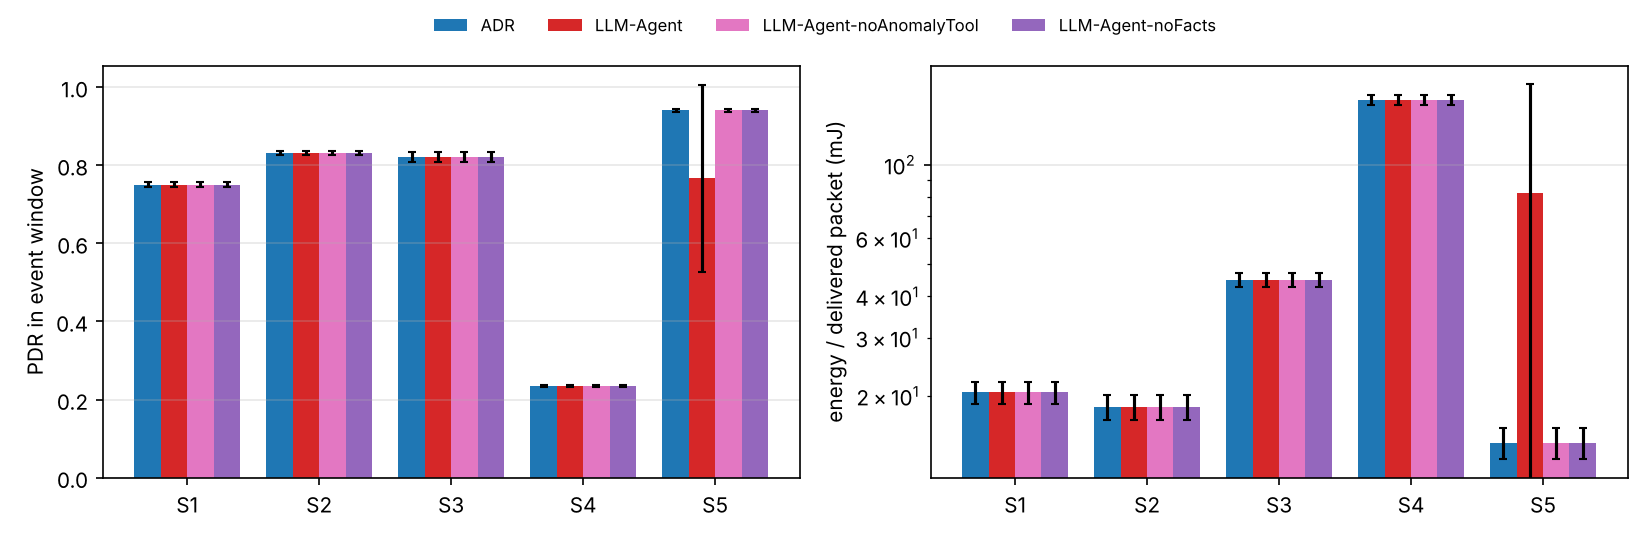
\includegraphics[width=\columnwidth]{../results/e6_ablations.png}
\caption{E6. Event-window PDR and energy per delivered packet for ADR, the full agent and the two
ablations (Qwen3-0.6B, 5 seeds).}
\label{fig:e6}
\end{figure}
